\subsection{Análise Quantitativa Complementar}

Além da avaliação qualitativa apresentada anteriormente, optou-se por incluir uma \emph{análise quantitativa complementar} utilizando algumas métricas de software identificadas na literatura~\cite{chidamber1994metrics, fenton2014software, gyimothy2005empirical, mccabe1976complexity}, descritas resumidamente a seguir:

\begin{enumerate}[(M1)]

\item{Line of Code (LoC)}

A métrica LoC é uma métrica tradicional para mensurar o tamanho físico de um software. Calcula-se nessa avaliação o número de linhas de código que cada sistema avaliado contém. Não são contabilizados documentações, comentários para explicar o que o código faz, nem as linhas em branco, segundo as observações de~\cite{fenton2014software}.

\item{Cyclomatic Complexity (CC)}

Métrica para medir a complexidade de um software e consiste basicamente em contar o número de caminhos diferentes que um método pode ter. É obtido através de heurísticas e independe da linguagem de programação.
Segundo o seu criador \emph{McCabe`s}~\cite{mccabe1976complexity}, é uma das métricas mais utilizadas para mensurar a complexidade de softwares (tanto para sistemas orientados a objetos quanto os procedurais).


\item{Weighted Methods Per Class (WMC)}

Mensura a complexidade das classes em termos da soma das complexidades dos métodos. De acordo com ~\cite{chidamber1994metrics}, o número de métodos de uma classe é uma forma efetiva para estimar o tempo e o esforços de manutenção para uma classe.


\item{Coupling Between Objects (CBO)}

Verifica o acoplamento entre objetos, ou seja, o nível de dependências entre as classes. Calcula-se aqui duas variáveis: o \emph{acoplamento eferente} (a quantidade de classes que uma classe depende) e; o \emph{acoplamento aferente} (a quantidade de classes que dependem de uma classe).

\item{Lack of Cohesion of Methods (LCOM)}

Avalia a falta de coesão entre os métodos de uma classe. Representa a diferença entre o número de pares de métodos de uma classe que não compartilham o mesmo conjunto de atributos e o número de pares que compartilham. Existem algumas variações dessa métrica. Nessa avaliação, o algoritmo utilizado é o LCOM1 de Chidamber \& Kemerer~\cite{chidamber1994metrics}.

\end{enumerate}


As métricas foram coletadas com a suíte de análise estática da empresa CoderGears\footnote{A suíte de ferramentas CodeGears está disponível no sítio \url{http://www.codergears.com}.} e com a ferramenta CLOC\footnote{A ferramenta CLOC está disponível no sítio \url{http://cloc.sourceforge.net}.}. Salienta-se que a justificativa para a seleção dessas métricas é verificar quantitativamente se o sistema modernizado no estudo de caso possui indicativos
de uma arquitetura melhor quando comparado com os demais sistemas da UnB, em termos de modularidade, coesão e acoplamento, atributos que podem segundo~\cite{fenton2014software}, contribuir na maximização da manutenibilidade dos sistemas de software. 

Nesse sentido, os sistemas selecionados para a análise estão listados na Tabela~\ref{sistemas_avaliados}. 

% Tabela dos sistemas para a avaliação
%======================================================================================
\begin{table}[!htb]
\centering
\small
\caption{Listagem dos sistemas avaliados.}
\label{sistemas_avaliados}
\begin{tabular}{|
>{\columncolor[HTML]{EFEFEF}}c |l|c|c|c|}
\hline
\cellcolor[HTML]{C0C0C0}\textbf{Sistema} & \multicolumn{1}{c|}{\cellcolor[HTML]{C0C0C0}\textbf{Descrição do Sistema}}                                 & \cellcolor[HTML]{C0C0C0}\textbf{\begin{tabular}[c]{@{}c@{}}Métrica    \\ LoC\end{tabular}} & \cellcolor[HTML]{C0C0C0}\textbf{\begin{tabular}[c]{@{}c@{}}Linguagem de \\ Programação\end{tabular}} & \cellcolor[HTML]{C0C0C0}\textbf{\begin{tabular}[c]{@{}c@{}}Desenvolvido\\ Em\end{tabular}} \\ \hline
\textbf{SAE}                             & Sistema de Estudo Socioeconômico                                                                           & 16087                                                                                      & VB                                                                                                   & 2000                                                                                       \\ \hline
\textbf{SAE}                             & Sistema de Estudo Socioeconômico                                                                           & 11078                                                                                      & C\#                                                                                                  & 2007                                                                                       \\ \hline
\textbf{SITAB}                           & Sistema de Tabelas de Apoio                                                                                & 14453                                                                                      & JAVA                                                                                                 & 2012                                                                                       \\ \hline
\textbf{SIADD}                           & Sistema de Avaliação de Docentes                                                                           & 39101                                                                                      & JAVA                                                                                                 & 2013                                                                                       \\ \hline
\textbf{SICONV}                          & Sistema de Convênios                                                                                       & 3796                                                                                       & JAVA                                                                                                 & 2014                                                                                       \\ \hline
\textbf{SIMAR}                           & Sistema de Materiais                                                                                       & 3213                                                                                       & JAVA                                                                                                 & 2015                                                                                       \\ \hline
\textbf{SAE}                             & \begin{tabular}[c]{@{}l@{}}Sistema de Estudo Socioeconômico\\ desenvolvido no estudo de caso.\end{tabular} & \textbf{9558}                                                                              & JAVA                                                                                                 & \textbf{2015}                                                                              \\ \hline
\end{tabular}
\end{table}



 
A métrica LoC pode ser visualizada na Tabela~\ref{sistemas_avaliados}. A Figura~\ref{fig:proporcao_tam_sae_versoes} mostra também um gráfico com as três versões do \acrshort{SAE}. As demais métricas coletadas estão disponíveis na Tabela~\ref{tab:coleta_metricas_sae}. Destaca-se que a granularidade da métrica LoC é por aplicação e as demais métricas é por classe ou componente (também chamado de \emph{entidade}) para obter mais informações sobre os sistemas e a sua arquitetura correspondente.

De acordo com a Figura~\ref{fig:proporcao_tam_sae_versoes}, as versões VB, C\# e Java do \acrshort{SAE} tem 16087, 11078, 9558 linhas de código respectivamente. A métrica LoC tem um propósito apenas informativo já que cada linguagem tem suas próprias características. Salienta-se que o novo \acrshort{SAE} é dividido em módulos \textit{back-end} (com os serviços de negócios) e o \textit{front-end} da aplicação (que ainda não está completo). O Código fonte completo pode ser consultado no sítio \url{https://github.com/erlangMS/samples/tree/master/sae/backend}.


% Figura que mostra o tamanho de cada versão do SAE
%======================================================================================

\begin{figure}[htb]
\centering
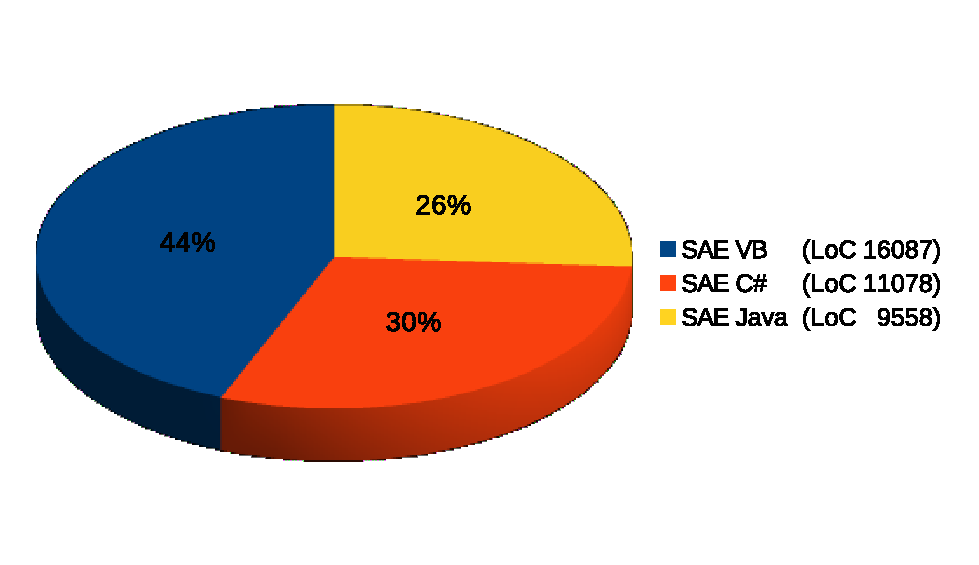
\includegraphics[scale=0.72]{/img/avaliacao/QP2/proporcao_tam_sae_versoes.eps}
\caption{Métrica LoC nas três versões do SAE.}
\label{fig:proporcao_tam_sae_versoes}
\end{figure}


Examinando a métrica WMC, percebe-se que os sistemas diferem nesse quesito. Tome como exemplo o \acrshort{SAE} Java com média WMC=8,17 em comparação ao \acrshort{SAE} VB com WMC=14,05 e o \acrshort{SAE} C\# com WMC=12,55. Segundo~\cite{chidamber1994metrics}, um valor médio até 10 é considerado bom e a partir disso, o sistema pode apresentar certa dificuldade em sua manutenção. Como se observa, a maior parte dos sistemas estão acima desse indicador ou apresentam alguma entidade acima deste valor, como indica a medição Max. Apenas como curiosidade, descobriu-se uma classe chamada \emph{VoEstudosSocioEconomicos} em C\# com 171 atributos, a qual os participantes decidiram refatorar em várias classes menores.

Analisando a complexidade ciclomática (métrica CC), verificou-se que o novo \acrshort{SAE} é muito parecido com o \acrshort{SAE} C\#. Segundo afirma~\cite{watson1996structured}, um valor até 10 é considerado bom e há boas razões para limitar essa complexidade ciclomática. Por exemplo, artefatos muito complexos são alvo de mais problemas, são difíceis entendê-los, testá-los e modificá-los. De acordo com esse limite, os sistemas \acrshort{SIADD}, \acrshort{SICONV} e o \acrshort{SIMAR}, provavelmente, precisariam ser revistos já que a complexidade ciclomática média foi ultrapassada. Todos os sistemas analisados tem alguma entidade que ultrapassou este limite, como por exemplo, o \acrshort{SIADD} com Max=322, o \acrshort{SICONV} com Max=109 e o \acrshort{SIMAR} com Max=123. 

Além disso, comparando os dados coletados da métrica LCOM, que mede a falta de coesão entre os métodos de uma classe, pode-se notar que o novo \acrshort{SAE} é o sistema mais coeso da lista. Para o \acrshort{SAE} C\#, foi pontuado o valor 0 para todas as entidades, podendo ser um erro ou limitação da ferramenta de análise estática na linguagem C\#. O princípio básico desta métrica é que as classes não devem ter muitas responsabilidades, limitando este valor na faixa entre 0 até 1. Valores altos apontam classes geralmente pouco coesas, como afirmam~\cite{chidamber1994metrics, gyimothy2005empirical}. Acredita-se que o design \acrshort{DDD} pode ter favorecido uma boa pontuação para o \acrshort{SAE} Java.

Do modo geral, o resultado obtido analisando as métricas de software 
nos sistemas selecionados indica que o novo sistema \acrshort{SAE} apresenta alguns
indicativos de uma melhora arquitetural, uma vez que as médias (Avg) e o desvio padrão (Std.) 
apontadas nas métricas coletadas são um pouco melhores no \acrshort{SAE} que nos
demais sistemas avaliados. No entanto, apenas com uma \emph{análise quantitativa}
não foi possível afirmar que a manutenibilidade poderia ser maximizada com 
o uso da abordagem proposta.


% Tabela de estatisticas coletadas
%======================================================================================
\begin{table}[!htb]
\centering
\caption{Coleta de estatísticas dos sistemas avaliados.}
\label{tab:coleta_metricas_sae}
\begin{tabular}{|c|c|c|c|c|c|c|}
\hline
\rowcolor[HTML]{C0C0C0} 
\cellcolor[HTML]{C0C0C0}                                                                                                      & \cellcolor[HTML]{C0C0C0}                                                                                     & \cellcolor[HTML]{C0C0C0}                                   & \multicolumn{4}{c|}{\cellcolor[HTML]{C0C0C0}\textbf{Estatísticas}}                             \\ \cline{4-7} 
\multirow{-2}{*}{\cellcolor[HTML]{C0C0C0}\textbf{\begin{tabular}[c]{@{}c@{}}Sistema / \\ Linguagem\end{tabular}}}             & \multirow{-2}{*}{\cellcolor[HTML]{C0C0C0}\textbf{\begin{tabular}[c]{@{}c@{}}Desenvolvido\\ em\end{tabular}}} & \multirow{-2}{*}{\cellcolor[HTML]{C0C0C0}\textbf{Métrica}} & \textit{\textbf{Avg}} & \textit{\textbf{Max}} & \textit{\textbf{Min}} & \textit{\textbf{Std.}} \\ \hline
\rowcolor[HTML]{EFEFEF} 
\cellcolor[HTML]{EFEFEF}{\color[HTML]{000000} }                                                                               & \cellcolor[HTML]{FFFFFF}                                                                                     & \textbf{CC}                                                & 7,10                  & 39,16                 & 0                     & 10,25                  \\ \cline{3-7} 
\cellcolor[HTML]{EFEFEF}{\color[HTML]{000000} }                                                                               & \cellcolor[HTML]{FFFFFF}                                                                                     & \textbf{WMC}                                               & 14,08                 & 65                    & 1                     & 13,84                  \\ \cline{3-7} 
\rowcolor[HTML]{EFEFEF} 
\cellcolor[HTML]{EFEFEF}{\color[HTML]{000000} }                                                                               & \cellcolor[HTML]{FFFFFF}                                                                                     & \textbf{LCOM}                                              & 0,85                  & 1                     & 0                     & 0,16                   \\ \cline{3-7} 
\rowcolor[HTML]{EFEFEF} 
\cellcolor[HTML]{EFEFEF}{\color[HTML]{000000} }                                                                               & \cellcolor[HTML]{FFFFFF}                                                                                     & \textbf{AC}                                                & 78,81                 & 1854                  & 0                     & 286,84                 \\ \cline{3-7} 
\multirow{-5}{*}{\cellcolor[HTML]{EFEFEF}{\color[HTML]{000000} \textbf{\begin{tabular}[c]{@{}c@{}}SAE \\ (VB)\end{tabular}}}} & \multirow{-5}{*}{\cellcolor[HTML]{FFFFFF}\textbf{2000}}                                                      & \textbf{EC}                                                & -                     & -                     & -                     & -                      \\ \hline
\rowcolor[HTML]{EFEFEF} 
\cellcolor[HTML]{EFEFEF}                                                                                                      & \cellcolor[HTML]{FFFFFF}                                                                                     & \textbf{CC}                                                & 3,78                  & 20                    & 1                     & 4,87                   \\ \cline{3-7} 
\cellcolor[HTML]{EFEFEF}                                                                                                      & \cellcolor[HTML]{FFFFFF}                                                                                     & \textbf{WMC}                                               & 12,55                 & 171                   & 1                     & 33,33                  \\ \cline{3-7} 
\rowcolor[HTML]{EFEFEF} 
\cellcolor[HTML]{EFEFEF}                                                                                                      & \cellcolor[HTML]{FFFFFF}                                                                                     & \textbf{LCOM}                                              & 0                     & 0                     & 0                     & 0                      \\ \cline{3-7} 
\rowcolor[HTML]{EFEFEF} 
\cellcolor[HTML]{EFEFEF}                                                                                                      & \cellcolor[HTML]{FFFFFF}                                                                                     & \textbf{AC}                                                & 0,54                  & 1                     & 0                     & 0,49                   \\ \cline{3-7} 
\multirow{-5}{*}{\cellcolor[HTML]{EFEFEF}\textbf{\begin{tabular}[c]{@{}c@{}}SAE WEB\\ (C\#)\end{tabular}}}                    & \multirow{-5}{*}{\cellcolor[HTML]{FFFFFF}\textbf{2007}}                                                      & \textbf{EC}                                                & 10,49                 & 25                    & 2                     & 5,31                   \\ \hline
\rowcolor[HTML]{EFEFEF} 
\cellcolor[HTML]{EFEFEF}                                                                                                      & \cellcolor[HTML]{FFFFFF}                                                                                     & \textbf{CC}                                                & 9,26                  & 153                   & 0                     & 12,66                  \\ \cline{3-7} 
\cellcolor[HTML]{EFEFEF}                                                                                                      & \cellcolor[HTML]{FFFFFF}                                                                                     & \textbf{WMC}                                               & 6,07                  & 93                    & 0                     & 7,02                   \\ \cline{3-7} 
\rowcolor[HTML]{EFEFEF} 
\cellcolor[HTML]{EFEFEF}                                                                                                      & \cellcolor[HTML]{FFFFFF}                                                                                     & \textbf{LCOM}                                              & 0,58                  & 1                     & 0                     & 0,37                   \\ \cline{3-7} 
\rowcolor[HTML]{EFEFEF} 
\cellcolor[HTML]{EFEFEF}                                                                                                      & \cellcolor[HTML]{FFFFFF}                                                                                     & \textbf{AC}                                                & 1,62                  & 48                    & 0                     & 4,13                   \\ \cline{3-7} 
\multirow{-5}{*}{\cellcolor[HTML]{EFEFEF}\textbf{\begin{tabular}[c]{@{}c@{}}SITAB WEB\\ (JAVA)\end{tabular}}}                 & \multirow{-5}{*}{\cellcolor[HTML]{FFFFFF}\textbf{2012}}                                                      & \textbf{EC}                                                & 8,71                  & 27                    & 0                     & 4,41                   \\ \hline
\rowcolor[HTML]{EFEFEF} 
\cellcolor[HTML]{EFEFEF}                                                                                                      & \cellcolor[HTML]{FFFFFF}                                                                                     & \textbf{CC}                                                & 19,89                 & 322                   & 0                     & 25,72                  \\ \cline{3-7} 
\cellcolor[HTML]{EFEFEF}                                                                                                      & \cellcolor[HTML]{FFFFFF}                                                                                     & \textbf{WMC}                                               & 16,66                 & 322                   & 0                     & 19,07                  \\ \cline{3-7} 
\rowcolor[HTML]{EFEFEF} 
\cellcolor[HTML]{EFEFEF}                                                                                                      & \cellcolor[HTML]{FFFFFF}                                                                                     & \textbf{LCOM}                                              & 0,79                  & 1                     & 0                     & 0,21                   \\ \cline{3-7} 
\rowcolor[HTML]{EFEFEF} 
\cellcolor[HTML]{EFEFEF}                                                                                                      & \cellcolor[HTML]{FFFFFF}                                                                                     & \textbf{AC}                                                & 3,53                  & 84                    & 0                     & 8,27                   \\ \cline{3-7} 
\multirow{-5}{*}{\cellcolor[HTML]{EFEFEF}\textbf{\begin{tabular}[c]{@{}c@{}}SIADD WEB\\ (JAVA)\end{tabular}}}                 & \multirow{-5}{*}{\cellcolor[HTML]{FFFFFF}\textbf{2013}}                                                      & \textbf{EC}                                                & 11,32                 & 323                   & 0                     & 17,16                  \\ \hline
\rowcolor[HTML]{EFEFEF} 
\cellcolor[HTML]{EFEFEF}                                                                                                      & \cellcolor[HTML]{FFFFFF}                                                                                     & \textbf{CC}                                                & 12,56                 & 109                   & 0                     & 19,87                  \\ \cline{3-7} 
\cellcolor[HTML]{EFEFEF}                                                                                                      & \cellcolor[HTML]{FFFFFF}                                                                                     & \textbf{WMC}                                               & 7,73                  & 71                    & 0                     & 11,11                  \\ \cline{3-7} 
\rowcolor[HTML]{EFEFEF} 
\cellcolor[HTML]{EFEFEF}                                                                                                      & \cellcolor[HTML]{FFFFFF}                                                                                     & \textbf{LCOM}                                              & 0,57                  & 1                     & 0                     & 0,36                   \\ \cline{3-7} 
\rowcolor[HTML]{EFEFEF} 
\cellcolor[HTML]{EFEFEF}                                                                                                      & \cellcolor[HTML]{FFFFFF}                                                                                     & \textbf{AC}                                                & 2,12                  & 32                    & 0                     & 4,68                   \\ \cline{3-7} 
\multirow{-5}{*}{\cellcolor[HTML]{EFEFEF}\textbf{\begin{tabular}[c]{@{}c@{}}SICONV WEB\\ (JAVA)\end{tabular}}}                & \multirow{-5}{*}{\cellcolor[HTML]{FFFFFF}\textbf{2014}}                                                      & \textbf{EC}                                                & 9,27                  & 35                    & 0                     & 7,25                   \\ \hline
\rowcolor[HTML]{EFEFEF} 
\cellcolor[HTML]{EFEFEF}                                                                                                      & \cellcolor[HTML]{FFFFFF}                                                                                     & \textbf{CC}                                                & 13,75                 & 123                   & 0                     & 24,83                  \\ \cline{3-7} 
\cellcolor[HTML]{EFEFEF}                                                                                                      & \cellcolor[HTML]{FFFFFF}                                                                                     & \textbf{WMC}                                               & 10,52                 & 68                    & 0                     & 15,80                  \\ \cline{3-7} 
\rowcolor[HTML]{EFEFEF} 
\cellcolor[HTML]{EFEFEF}                                                                                                      & \cellcolor[HTML]{FFFFFF}                                                                                     & \textbf{LCOM}                                              & 0,52                  & 1                     & 0                     & 0,34                   \\ \cline{3-7} 
\rowcolor[HTML]{EFEFEF} 
\cellcolor[HTML]{EFEFEF}                                                                                                      & \cellcolor[HTML]{FFFFFF}                                                                                     & \textbf{AC}                                                & 1,54                  & 13                    & 0                     & 2,82                   \\ \cline{3-7} 
\multirow{-5}{*}{\cellcolor[HTML]{EFEFEF}\textbf{\begin{tabular}[c]{@{}c@{}}SIMAR WEB\\ (JAVA)\end{tabular}}}                 & \multirow{-5}{*}{\cellcolor[HTML]{FFFFFF}\textbf{2015}}                                                      & \textbf{EC}                                                & 8,94                  & 39                    & 0                     & 8,00                   \\ \hline
\rowcolor[HTML]{EFEFEF} 
\cellcolor[HTML]{EFEFEF}                                                                                                      & \cellcolor[HTML]{FFFFFF}                                                                                     & \textbf{CC}                                                & 7,38                  & 42                    & 0                     & 7,08                   \\ \cline{3-7} 
\cellcolor[HTML]{EFEFEF}                                                                                                      & \cellcolor[HTML]{FFFFFF}                                                                                     & \textbf{WMC}                                               & 8,17                  & 32                    & 0                     & 5,65                   \\ \cline{3-7} 
\rowcolor[HTML]{EFEFEF} 
\cellcolor[HTML]{EFEFEF}                                                                                                      & \cellcolor[HTML]{FFFFFF}                                                                                     & \textbf{LCOM}                                              & 0,38                  & 1                     & 0                     & 0,40                   \\ \cline{3-7} 
\rowcolor[HTML]{EFEFEF} 
\cellcolor[HTML]{EFEFEF}                                                                                                      & \cellcolor[HTML]{FFFFFF}                                                                                     & \textbf{AC}                                                & 2,50                  & 16                    & 0                     & 2,58                   \\ \cline{3-7} 
\multirow{-5}{*}{\cellcolor[HTML]{EFEFEF}\textbf{\begin{tabular}[c]{@{}c@{}}SAE WEB\\ (JAVA)\end{tabular}}}                   & \multirow{-5}{*}{\cellcolor[HTML]{FFFFFF}\textbf{2015}}                                                      & \textbf{EC}                                                & 9,44                  & 23                    & 1                     & 4,49                   \\ \hline
\end{tabular}
\end{table}





